\documentclass[12pt]{article}
\usepackage[utf8]{inputenc}
\usepackage{indentfirst}
\usepackage{graphicx}

\graphicspath{{~/path/to/file}}

\usepackage[colorlinks=true, citecolor=blue, pagecolor=blue,
  linkcolor=blue, menucolor=blue, urlcolor=blue, frenchlinks=True, breaklinks]{hyperref}

\title{ResBaz Live demo}
\author{Chun Ly}
\date{May 2020}

% This is just a commit to demonstrate git

\begin{document}

\maketitle

\section{Introduction}

\textit{Lorem ipsum dolor sit amet, consectetur adipiscing elit, sed do eiusmod tempor incididunt ut labore et dolore magna aliqua. Ut enim ad minim veniam, quis nostrud exercitation ullamco laboris nisi ut aliquip ex ea commodo consequat. Duis aute irure dolor in reprehenderit in \emph{voluptate velit esse cillum dolore} eu fugiat nulla pariatur. Excepteur sint occaecat cupidatat non proident, sunt in culpa qui officia deserunt mollit anim id est laborum.}

\noindent This is a new paragraph that is automatically indented.
This sentence is still part of the same paragraph since I only had \underline{one} carriage return.
This is more text\\~\\
{\Large REsBAz Rules}
\large{RESBAZ RULES}
\textsc{Resbaz Rules}
\textsf{This is normal text}

\begin{flushright}
    This is centered text, and remains centered until it reaches the end of the environment.
    
    Lorem ipsum dolor sit amet, consectetur adipiscing elit, sed do eiusmod tempor incididunt ut labore et dolore magna aliqua. Ut enim ad minim veniam, quis nostrud exercitation ullamco laboris nisi ut aliquip ex ea commodo consequat. Duis aute irure dolor in reprehenderit in \emph{voluptate velit esse cillum dolore} eu fugiat nulla pariatur. Excepteur sint occaecat cupidatat non proident, sunt in culpa qui officia deserunt mollit anim id est laborum.
\end{flushright}

\flushright{a;slkdjfbasdlkfj ;laksdjfkl;}
\flushleft{text below that is flushed right}

We provide an overview in Section \ref{sec:overview} and describe our dataset in
Section \ref{sec:data}.

\section{Another section}

\newpage
\section{This is my first section in my paper}
\label{sec:overview}

\subsection{... my first sub-section under my first section}
\label{sec:data}

The linear equation, $y = m\sin{(x/\pi)} + b$, is used to fit the data.
This yielded a best fit of $m = 0.95$ and $b = 0.25$.
Einstein's famous equation is:
$$E \neq m_0 c^{2x}$$

See Eq \ref{eq1}

\begin{equation}
\frac{{\rm SFR}}{M_{\odot}~{\rm yr}^{-1}} =
4.4\times10^{-42} \cdot \frac{L({\rm H}\alpha)}{{\rm erg}~{\rm s}^{-1}}
\label{eq1}
\end{equation}
~\\

%booktabs

\begin{tabular}{c | l r}
                 & Post-scarcity & Austerity \\ \hline
techno-optimist  & Star Trek     & Robocop   \\
techno-pessimist & Matrix        & Terminator \\
\end{tabular}

\clearpage

\begin{figure}[h]
    \centering
    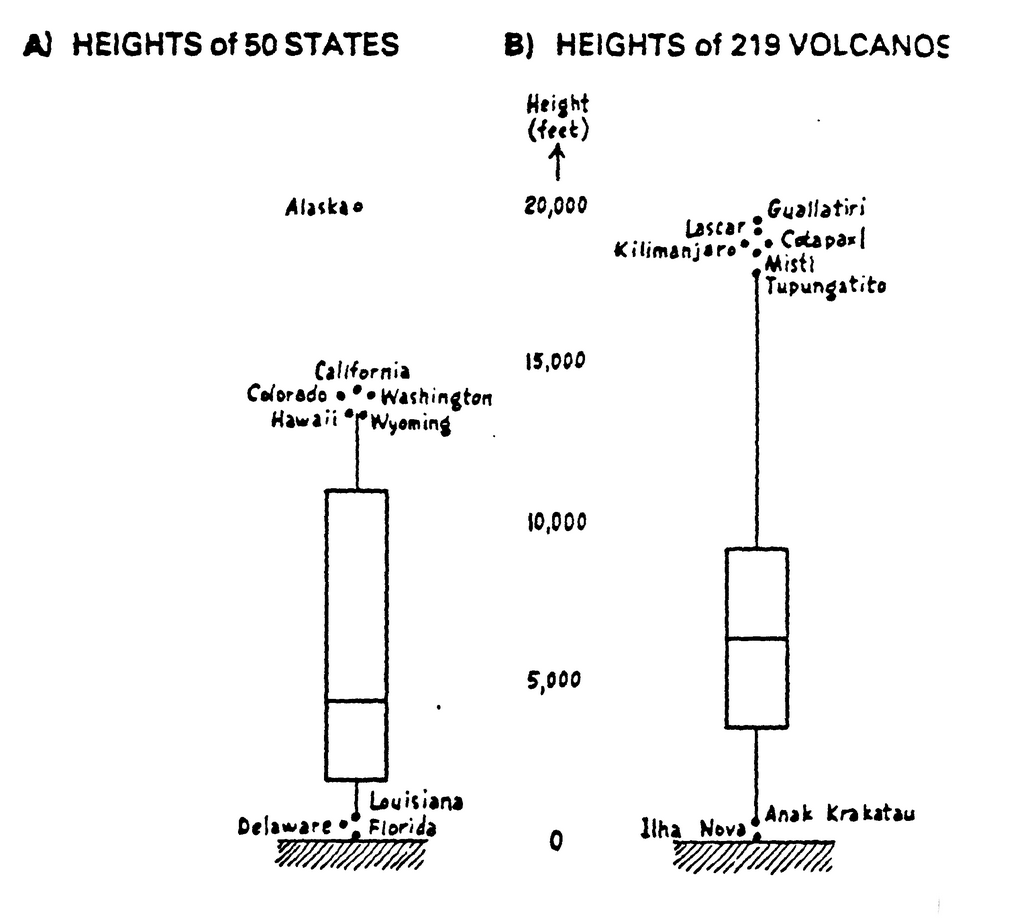
\includegraphics[width = .5\textwidth]{tables-plots/tukey.png}
    \caption{Early box and whiskers plots}
    \label{fig:tukeysketch}
\end{figure}

\clearpage

See figure \ref{fig:tukeysketch}

\begin{table}[t]
    \centering
    \doublespacing % Note that this means you should declare the setspace package in any document including this table
               % (included only for aesthetic purposes)
\begin{tabular}{c|l l} % Vertical bars give lines, which people don't appreciate for some reason. 
                       % alignment options for each column: c = center, l = left, r = right  
                 & Post-scarcity  & Austerity \\ \hline % There are fancier ways to make a horizontal line, see below
Techno-optimist  & Star Trek      & Robocop    \\ % Line breaks are required, as they define rows
Techno-pessimist & Matrix         & Terminator \\
% The alignments above are for readability only. They are unnecessary for compiling.
\end{tabular}

% For fancier tables, use the popular booktabs package, which includes weighted lines in the \toprule, \midrule, \bottomrule commands.
    \caption{The Future}
    \label{tab:futures}
\end{table}

\end{document}
